\section{Introduction}

For the modern programmer, development has progressed beyond just writing code in a text editor and now increasingly involves conversing with a wide-variety of programming tools. As incremental changes are made, type checkers, debuggers, interpreters, program synthesizers and so forth all provide feedback which seeks to increase programmer productivity or ensure program correctness. Unfortunately, however, programming languages typically only assign meaning to programs which are already fully-formed and well-typed. As a result, these tools struggle to deal with what is perhaps one of the most common states of a program during development: an unfinished piece of work with ongoing editing or as-yet-unresolved semantic errors. Throughout the editing process then, feedback from these tools is only available sporadically, limiting their usefulness when they are needed most.

This troublesome issue, where programming tools have gaps in their services throughout the editing process, is aptly known as the \emph{gap problem}. Previously, most attempts to close such gaps have relied on \textit{ad hoc} or fragile heuristics, for example, making assumptions about missing tokens, or ignoring large swathes of invalid code all together \cite{DBLP:conf/oopsla/KatsJNV09, DBLP:conf/snapl/OmarVHSGAH17}. Recently though, the work of  \cite{DBLP:conf/snapl/OmarVHSGAH17} has outlined a more principled approach: rather than treating intermediate edit states as meaningless, one can extend a language's syntax and semantics to explicitly represent such states as well-formed terms. Every editor state can then be assigned static or even dynamic meaning, allowing programming tools to handle them in a uniform way and removing the need for such \emph{ad hoc} heuristics.

To varying degree, systems including Haskell \cite{GHCHoles}, Idris \cite{DBLP:journals/jfp/Brady13}, Agda \cite{DBLP:conf/icfp/Norell13}, and Hazel \cite{DBLP:conf/popl/OmarVHAH17} implement this approach through a feature known as \emph{typed-holes}. When a program has a missing syntactic piece, rather than treating the entire program as meaningless, we localize the issue by inserting an \emph{empty hole} expression at the unfinished location. Likewise, semantically inconsistent expressions, e.g. those that are ill-typed or reference undefined identifiers, may be wrapped with a \emph{non-empty hole} expression, isolating the inconsistency from the program at large. Tools can then the aid the developer by providing static information about these holes - displaying the variables and types in scope, inferring the expected type, or even synthesizing possible hole-fillings \cite{DBLP:conf/haskell/Gissurarson18, DBLP:journals/pacmpl/LubinCOC20}. 

\begin{figure}
	\centering
	\subcaptionbox{Empty and non-empty holes\label{fig:arith-initial}}{
		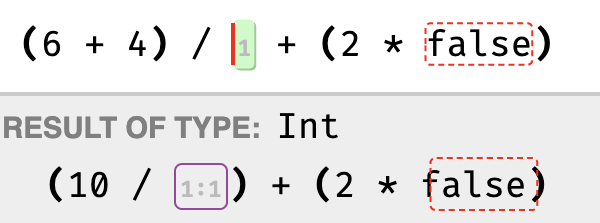
\includegraphics[scale=0.47,valign=t]{imgs/arith-initial.png}%
		\vphantom{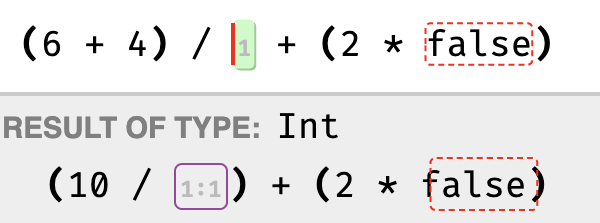
\includegraphics[scale=0.47,valign=t]{imgs/arith-initial.png}}
	}
	\hfil
	\subcaptionbox{Result after filling empty hole\label{fig:arith-partial}}{
		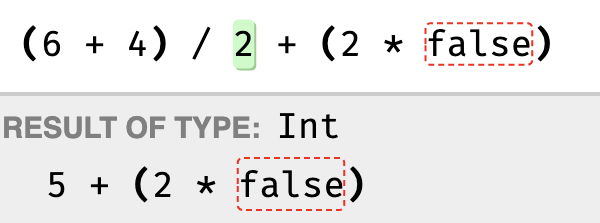
\includegraphics[scale=0.47,valign=t]{imgs/arith-partial.png}%
	 	\vphantom{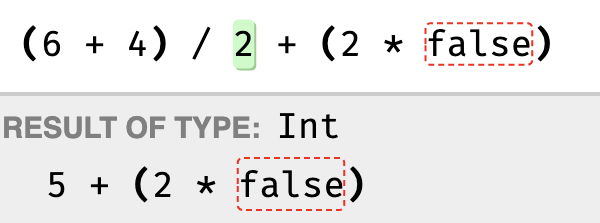
\includegraphics[scale=0.47,valign=t]{imgs/arith-partial.png}}
	}
	\hfil\par\bigskip
	\subcaptionbox{Result after filling non-empty hole\label{fig:arith-complete}}{
		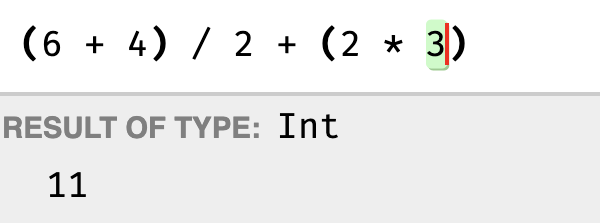
\includegraphics[scale=0.47,valign=t]{imgs/arith-complete.png}
	}
	\caption{Live Evaluation with Expression Holes}
	\label{fig:arith-example}
\end{figure}

Most notable among the aforementioned systems is Hazel - a structure editor which was designed from logical and type-theoretic first principles to seamlessly and fully-automatically insert holes throughout the editing process. Starting from an empty hole, every possible program can be built up using a set of edit actions which directly manipulate the syntax tree. Along the way, Hazel maintains a \emph{maximal liveness} invariant so that every intermediate step is a valid term with well-defined static and dynamic semantics, completely eliminating the gap problem \cite{DBLP:journals/pacmpl/OmarVCH19}. \autoref{fig:arith-example} displays screenshots of a small part of the Hazel editor, with the user in the process of editing a simple arithmetic expression. Considering only Fig.~\ref{fig:arith-initial} for now, both variants of typed-holes are present: an empty hole labeled with id \li{1} indicates a missing piece of the expression, and a non-empty hole, shown as a dashed red box, serves as a membrane around the type inconsistency related to the term \li{false}.

One of the main contributions of Hazel is its comprehensive dynamic semantics which allows evaluation to continue "around holes" \cite{DBLP:journals/pacmpl/OmarVCH19}. This stands in contrast to systems such as Haskell, which, when supplied with appropriate compiler flags, treat holes as panics - reminiscent of a common pattern where developers raise an exception at yet-to-be-implemented code locations \cite{GHCHoles}. With Hazel, however, upon evaluation encountering a hole, rather than panicking or otherwise terminating the program, Hazel defers the evaluation of that particular expression and those that rely on. It then continues to evaluate all other complete (i.e. hole-less) parts of the program as much as possible. Finally, evaluation pauses, yielding an \emph{indeterminate} result if there are still holes present. At a later time, the remaining holes in this indeterminate result can be filled, and evaluation resumes without having to restart the program. 

The rest of \autoref{fig:arith-example} demonstrates this live evaluation. Initially, the expression shown in Fig.~\ref{fig:arith-initial} contains two holes. Hazel partially evaluates the expression, reducing the complete term \li{6 + 4} to \li{10}, but can perform no further reductions. An indeterminate result is displayed, still containing both holes present in the initial expression. In Fig.~\ref{fig:arith-partial}, we then fill the empty hole with id \li{1} using the value \li{5}. This allows evaluation to resume, further reducing \li{(6 + 4) / 2} to \li{5}, but again pausing due to the presence of the non-empty hole. Finally, in Fig.~\ref{fig:arith-complete}, we resolve the typing inconsistency by replacing the term \li{false} with the integer \li{3}. The non-empty hole is automatically removed, and Hazel now produces a concrete value \li{11}. At no point during this process is the editor state meaningless, nor is the program ever restarted.

While Hazel itself is still under development, and is currently little more than a lambda calculus with primitive types, sums, and products, it seeks to soon reach feature-parity with production-level languages such as Elm \cite{DBLP:conf/pldi/CzaplickiC13, Elm, DBLP:journals/pacmpl/OmarVCH19}. Indeed, the machinery behind Hazel is not limited to its specific features, but rather, it provides a systematic, near-mechanical way to build similar structure editors for any language. Its semantics are built up using common techniques from gradual typing \cite{DBLP:conf/snapl/SiekVCB15}: holes are considered to have the unknown type, and terms are elaborated into a cast calculus to handle such typing at runtime. Additional machinery from contextual modal type theory \cite{DBLP:journals/tocl/NanevskiPP08} is then used to track substitutions which occur around holes, allowing holes to be filled in any order while producing the same final result. Given this principled theoretical basis, future work may even allow us to algorithmically generate such structure editors in a fully automatic way, developing something akin to the Gradualizer \cite{DBLP:conf/popl/CiminiS16}. However, for any of this to be possible, and indeed to apply these techniques to any full-fledged functional programming language at all, one commonplace feature still needs more careful consideration: \emph{pattern matching}.